\section{研究内容}\label{se3}
本章では,概要,開発環境,関連研究,システム概要を述べた後に,開発した本プラットフォームの詳細について述べる.

\subsection{概要}
本研究の目的は,情報倫理教育に関する学習を支援することである.そのため,学習者が情報倫理に関して学ぶ際手軽に学習する環境を構築する必要がある.これを解決するために本研究では学習をインターネット上で手軽に学習するためにwebアプリケーションを用いて本プラットフォームを開発した.
本プラットフォームは,情報倫理に関して学習する学習者と情報倫理に関するコンテンツを提供する教材提供者を対象としたシステムである.教材提供者に対して本プラットフォームではコンテンツ提供機能,統計情報提供機能,コンテナ管理機能を用意している.
教材提供者はこれらの機能を用いることにより情報倫理に関するコンテンツをwebアプリケーション上に投稿でき,学習者はそれらのコンテンツを用いて情報倫理に関する学習を行える.

\subsection{開発環境}
本プラットフォームを作成するにあたって使用したPCのスペックと開発環境を表\ref{env}に示す.

\begin{table}[htb]
    \begin{center}
        \caption{PCのスペックと開発環境}
        \begin{tabular}{|l|l|} \hline
            CPU & Intel Core i7 @ 3.70GHz \\ \hline
            Memory &  24.0GB \\ \hline
            OS & Windows 10 Education 64-bit \\ \hline
            開発環境 & 
            \begin{tabular}{l}
            Docker version 20.10.0, build 7287ab3 \\ docker-compose version 1.27.4, build 40524192
            \end{tabular}\\ \hline
        \end{tabular}
        \label{env}
    \end{center}
\end{table}

\subsubsection{クライアントシステムとサーバシステムの開発環境}
クライアントシステムとサーバシステムの開発にはDockerを用いた.表\ref{client},表\ref{server}にそれぞれの開発環境を示す.

\begin{table}[htb]
    \begin{center}
        \caption{クライアントシステムの開発環境}
        \begin{tabular}{|l|l|} \hline
            OS & Linux \\ \hline
            使用言語 & 
            \begin{tabular}{l}
            Python 3.7.9 \\ Django 3.0.2 \\
            \end{tabular}\\ \hline
        \end{tabular}
        \label{client}
    \end{center}
\end{table}

\begin{table}[htb]
    \begin{center}
        \caption{サーバシステムの開発環境}
        \begin{tabular}{|l|l|} \hline
            OS & GNU/Linux \\ \hline
            使用言語 & 
            \begin{tabular}{l}
            go version go1.15.6 linux/amd64 \\ djangorestframework 3.12.1 \\ 
            \end{tabular}\\ \hline
        \end{tabular}
        \label{server}
    \end{center}
\end{table}
\newpage
\subsection{関連研究}
関連研究として,上田氏らの「倫倫姫プロジェクト-学人連携Moodleによる多言語情報倫理eラーニング-」\cite{rinri}がある.

倫倫姫プロジェクトでは大学の情報倫理教育における以下3つの問題を解決している.

\begin{enumerate}[(i)]
    \item 標準化と可視化がなされていない \label{i}
    \item 留学生への教育が困難 \label{ii}
    \item 持続可能性が低い \label{iii}
\end{enumerate}

(\ref{i})を解決するために,倫倫姫ではサンプル規程集「A3301 教育テキスト作成ガイドライン(一般利用者向け)」に準拠することで,内容を標準化した.
また,受講履歴を閲覧でき受講者の学習状況の可視化も実現した.

(\ref{ii})を解決するために,倫倫姫では英語,中国語,韓国版を作成しており,各言語圏の文化の違いも考慮しコンテンツを作成することで解決した.

(\ref{iii})を解決するために,倫倫姫ではSCORMが規定するeラーニングコンテンツパッケージを利用した.
これは,パッケージ構造とリソースを記述するマニフェストファイル(imsmanifest.xml)とそれから参照される物理ファイル(HTML,swfなど)をファイル単位で修正可能なため継続的な改訂を可能としている.

\subsection{システム概要}
\subsubsection{要件定義}
本システムはサーバ,クライアントで以下の要件を持たす必要がある.

まずサーバの要件を示す.

\begin{itemize}
    \item Dockerの動作: すべての開発にDockerを用いる
    \item Webサーバの動作: Webアプリケーションの公開に用いる
    \item Pythonの動作: Djangoの動作に用いる
    \item Goの動作: APIの動作に用いる
    \item PostgreSQLの動作: ユーザの管理等のデータベースとして用いる
\end{itemize}

サーバはWebサーバを用いてクライアントをネットワークに公開し,Dockerを用いてPythonとGoとPostgreSQLを動作させる.
PythonはDjangoを動作させ,クライアントにGUI等を提供する.
GoはAPI作成に用いて,Dockerを操作する.
PostgreSQLは,Djangoを通してクライアントから入力されたデータ等を保存する.

続いて,クライアントの要件を示す.

\begin{itemize}
    \item html5が解釈できるWebブラウザの動作: クライアントの動作環境となる 
\end{itemize}

クライアントはWebアプリケーションであり,html5で記述されている.
クライアントは教材提供者と学習者に対してGUIを提供する.
詳細は,\ref{sec:fun1}節,\ref{sec:fun2}節,\ref{sec:fun3}節で述べる.

また,コンテンツ提供機能は日々変化する情報倫理に対応するため,コンテンツを素早く投稿,編集する必要があるため作成した.
統計情報提供機能は,年代,性別の違いから情報倫理に関する意識に違いが生まれていることから作成した.
コンテナ管理機能は,教材提供者が過去に作成したアプリケーションを用いたい場合があるため作成した.

\newpage
\subsubsection{システム構成}
本システムの構成を図\ref{system}に示す.本システムはDjangoで構成されるアプリケーション部(以下,クライアント),およびGoとdjangorestframeworkで構成されるサーバ部(以下,サーバ)から構築される.
サーバはAPIを用いて統計情報提供機能とコンテナ管理機能を動作させる.

\begin{figure}[htbp]
    \begin{center}
        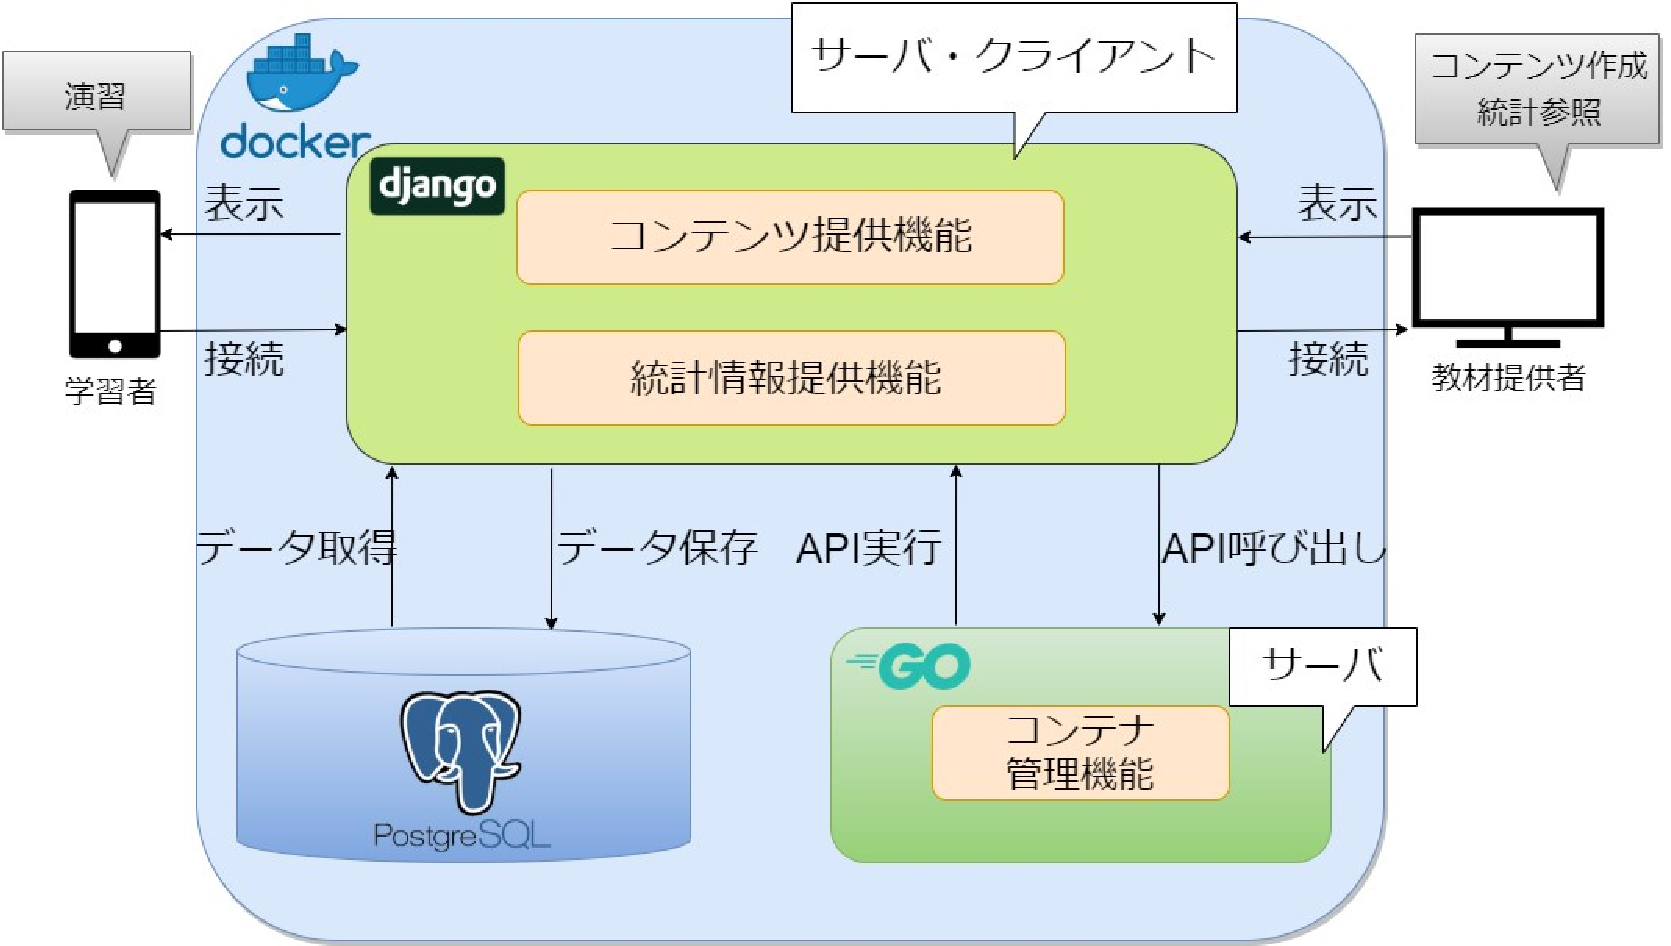
\includegraphics[width=18cm,height=17cm,keepaspectratio]{system-crop.pdf}\\
        %includegraphicsの詳しい使い方ははLaTeXの参考書を参照.
    \end{center}
    \caption{システム構成}
    \label{system}
\end{figure}


コンテンツ提供機能のGUIを図\ref{teikyou}に,統計情報提供機能のGUIを図\ref{toukei}に,コンテナ管理機能のGUIを図\ref{kanri}にそれぞれ示す.

\newpage
教材提供者は図\ref{teikyou}のコンテンツ提供機能を用いて情報倫理に関するコンテンツを提供する.

\begin{figure}[htbp]
    \begin{center}
        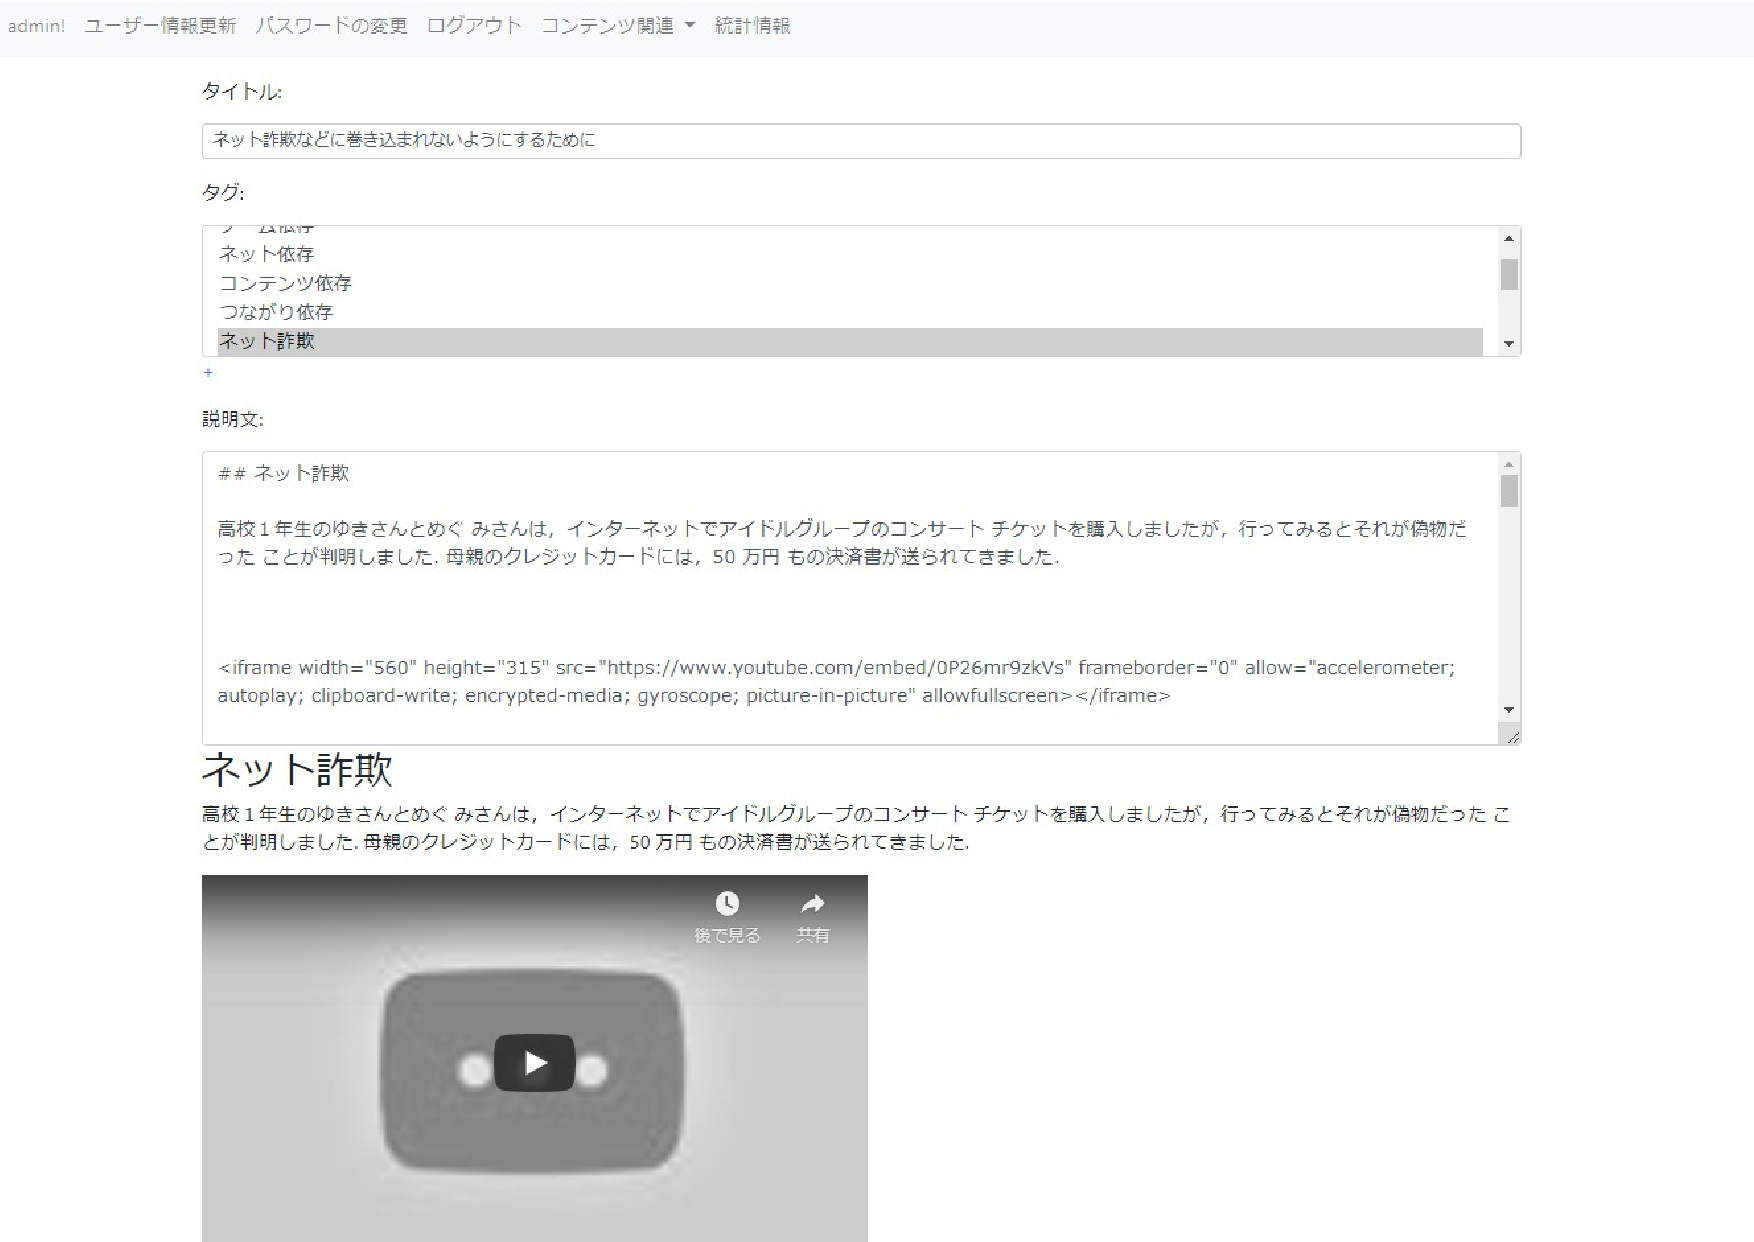
\includegraphics[width=18cm,height=17cm,keepaspectratio]{create_content-crop.pdf}\\
        %includegraphicsの詳しい使い方ははLaTeXの参考書を参照.
    \end{center}
    \caption{コンテンツ提供機能のGUI}
    \label{teikyou}
\end{figure}

\newpage
図\ref{toukei}の統計情報提供機能では,教材提供者が学習者の回答情報等をグラフとして確認できる.
\begin{figure}[htbp]
    \begin{center}
        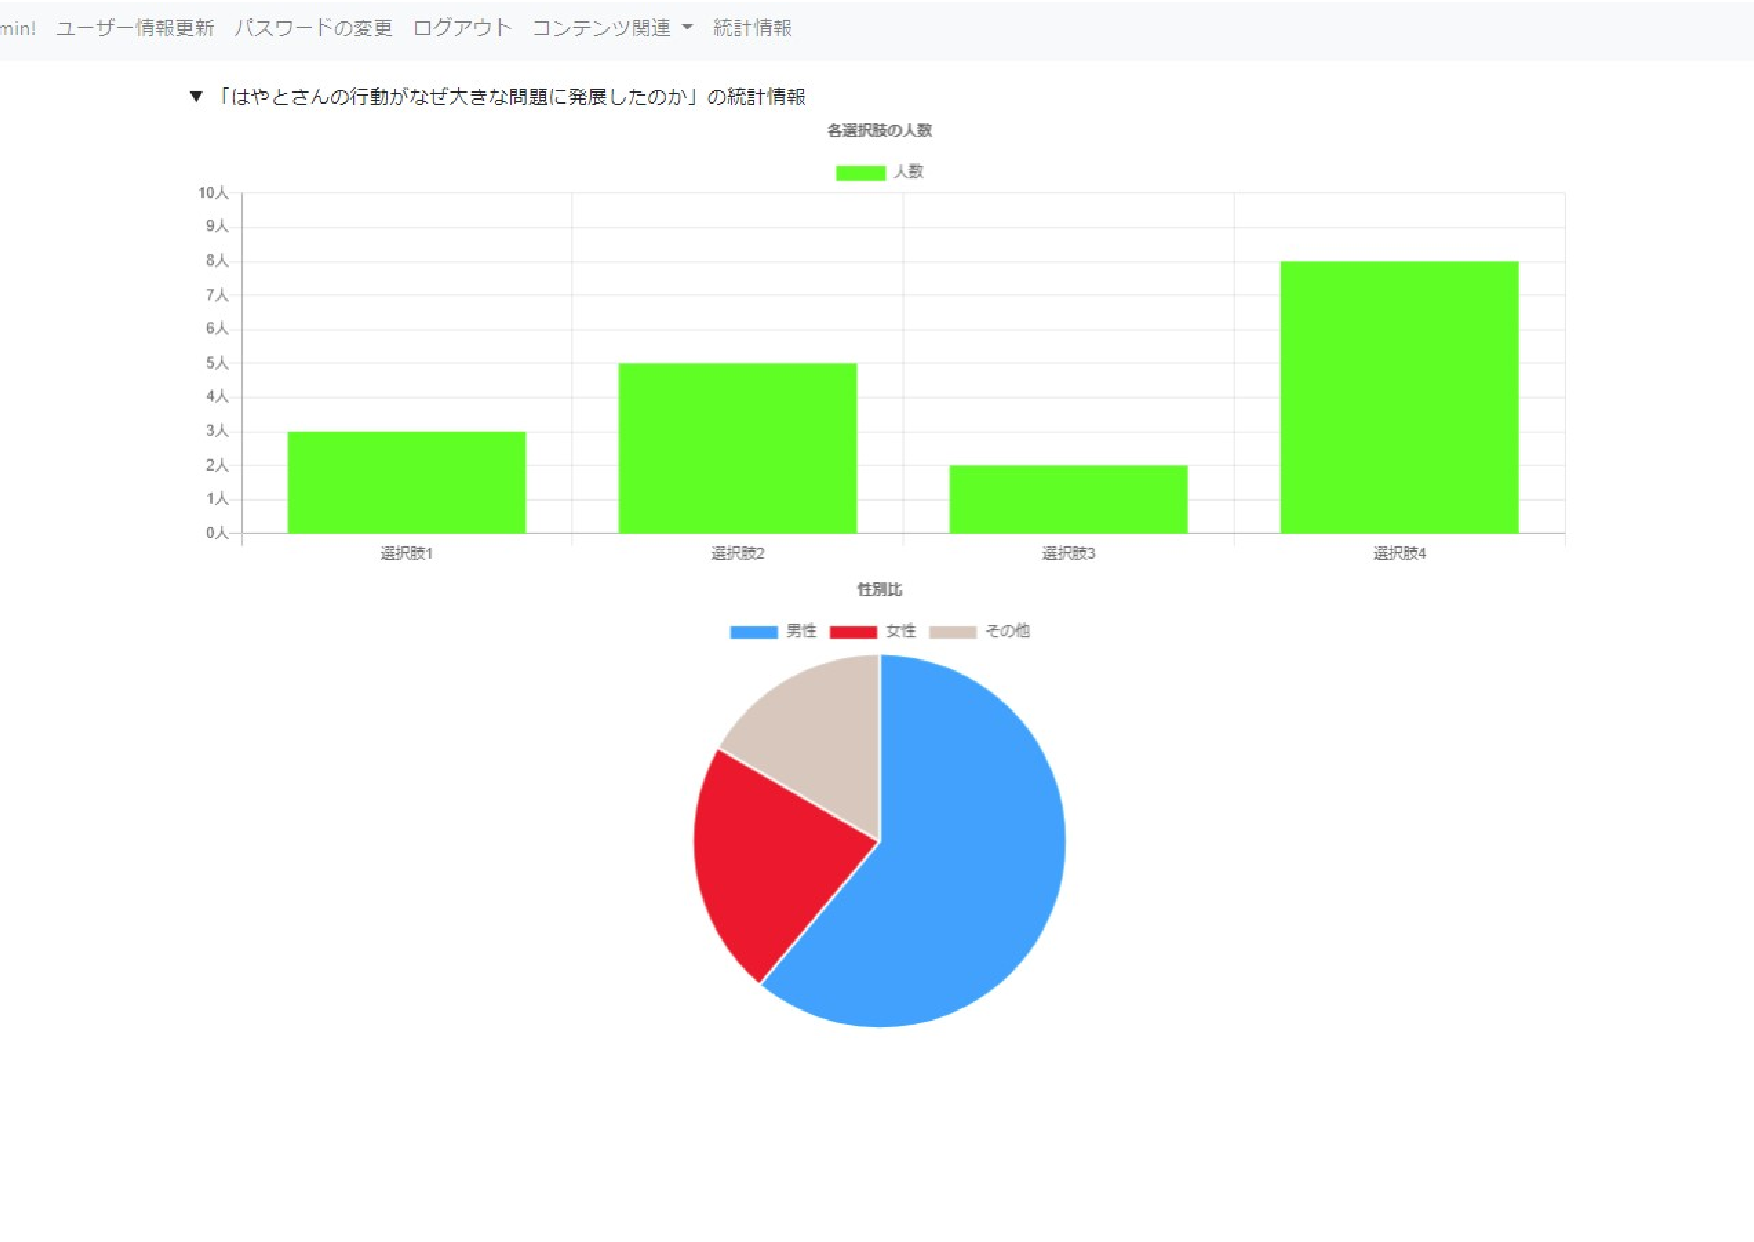
\includegraphics[width=18cm,height=17cm,keepaspectratio]{toukei-crop.pdf}\\
        %includegraphicsの詳しい使い方ははLaTeXの参考書を参照.
    \end{center}
    \caption{統計情報提供機能のGUI}
    \label{toukei}
\end{figure}

\newpage
図\ref{kanri}のコンテナ管理機能では教材提供者がDockerを用いて作成した他の教育アプリケーションを本プラットフォームでも利用することが可能となる.
\begin{figure}[htbp]
    \begin{center}
        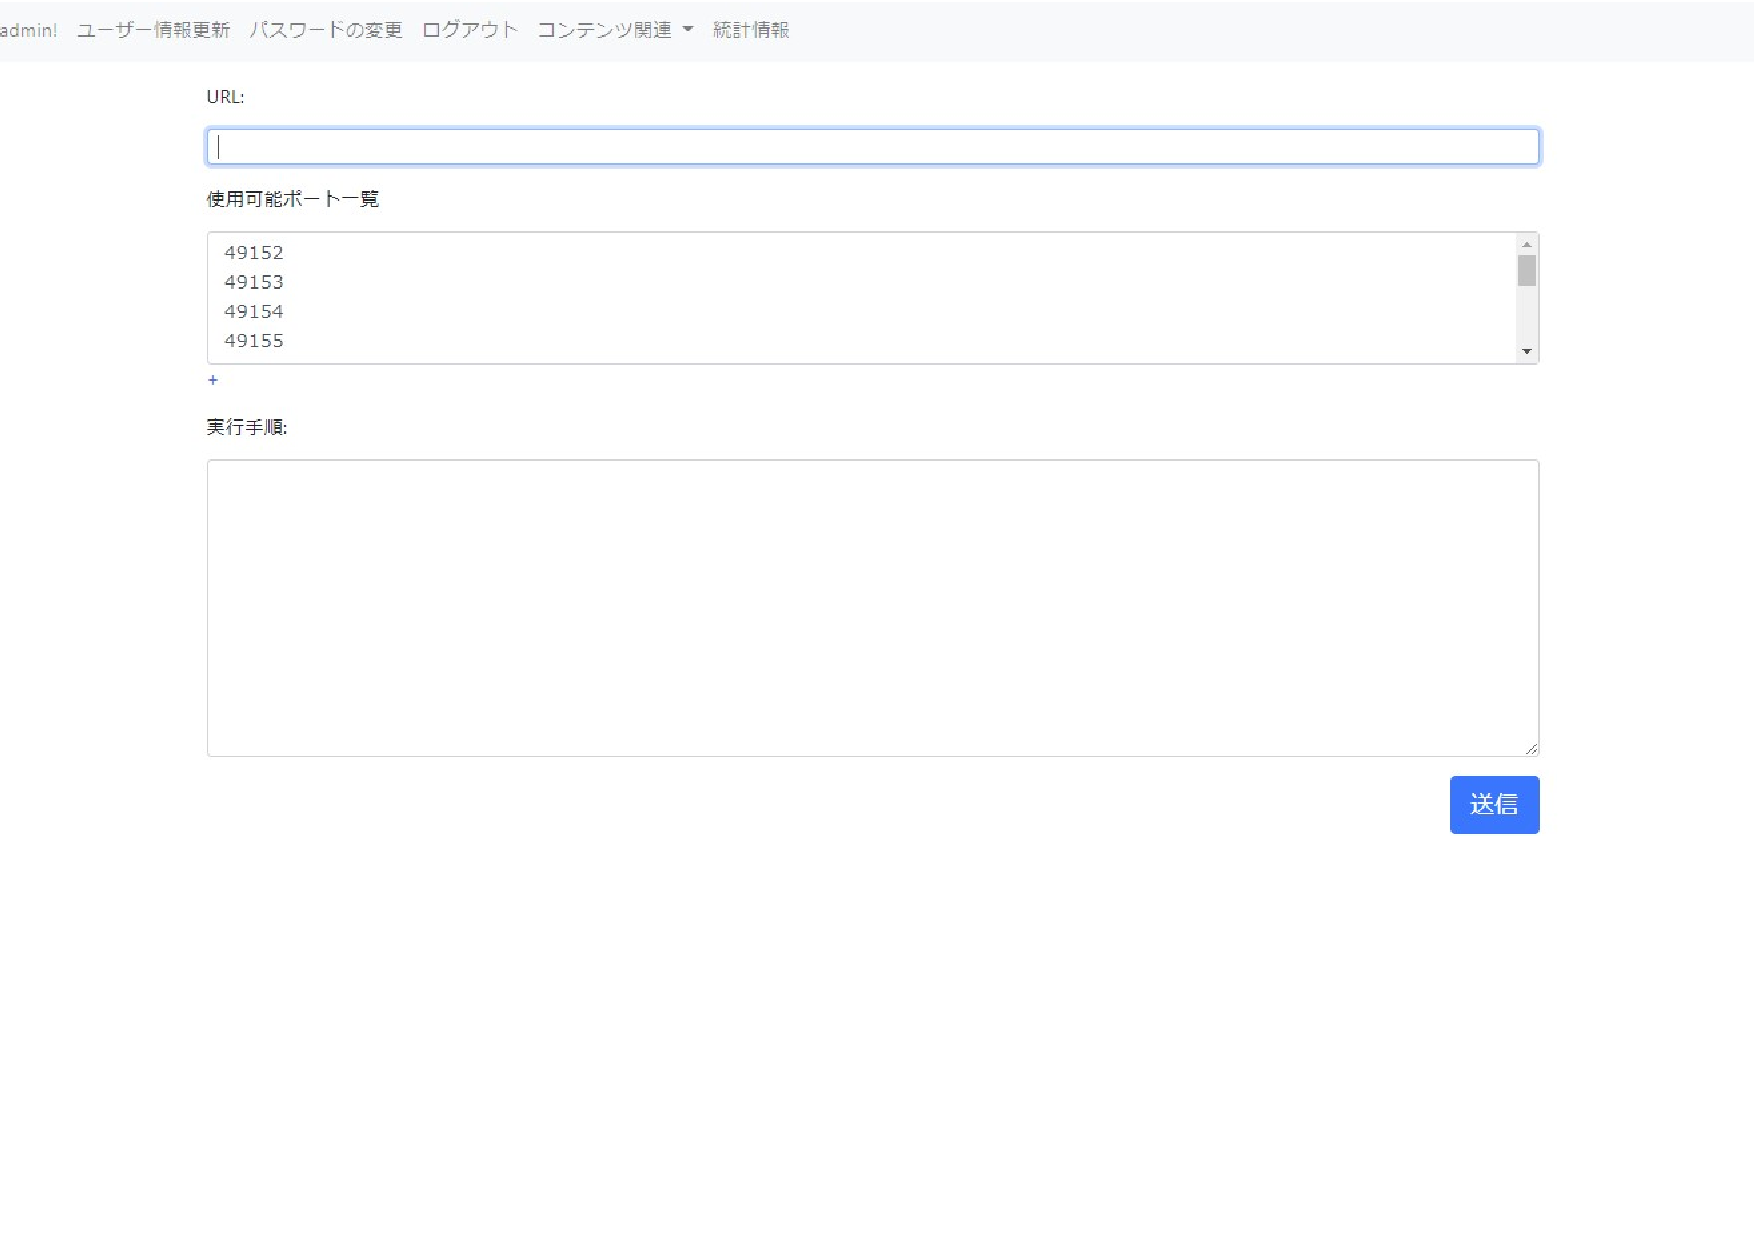
\includegraphics[width=18cm,height=17cm,keepaspectratio]{container_management-crop.pdf}\\
        %includegraphicsの詳しい使い方ははLaTeXの参考書を参照.
    \end{center}
    \caption{コンテナ管理機能のGUI}
    \label{kanri}
\end{figure}

\newpage
学習者は図\ref{teikyou}のコンテンツ提供機能を用いて作成されたコンテンツを図\ref{naiyou}のようにして閲覧,学習することが可能である.
\begin{figure}[htbp]
    \begin{center}
        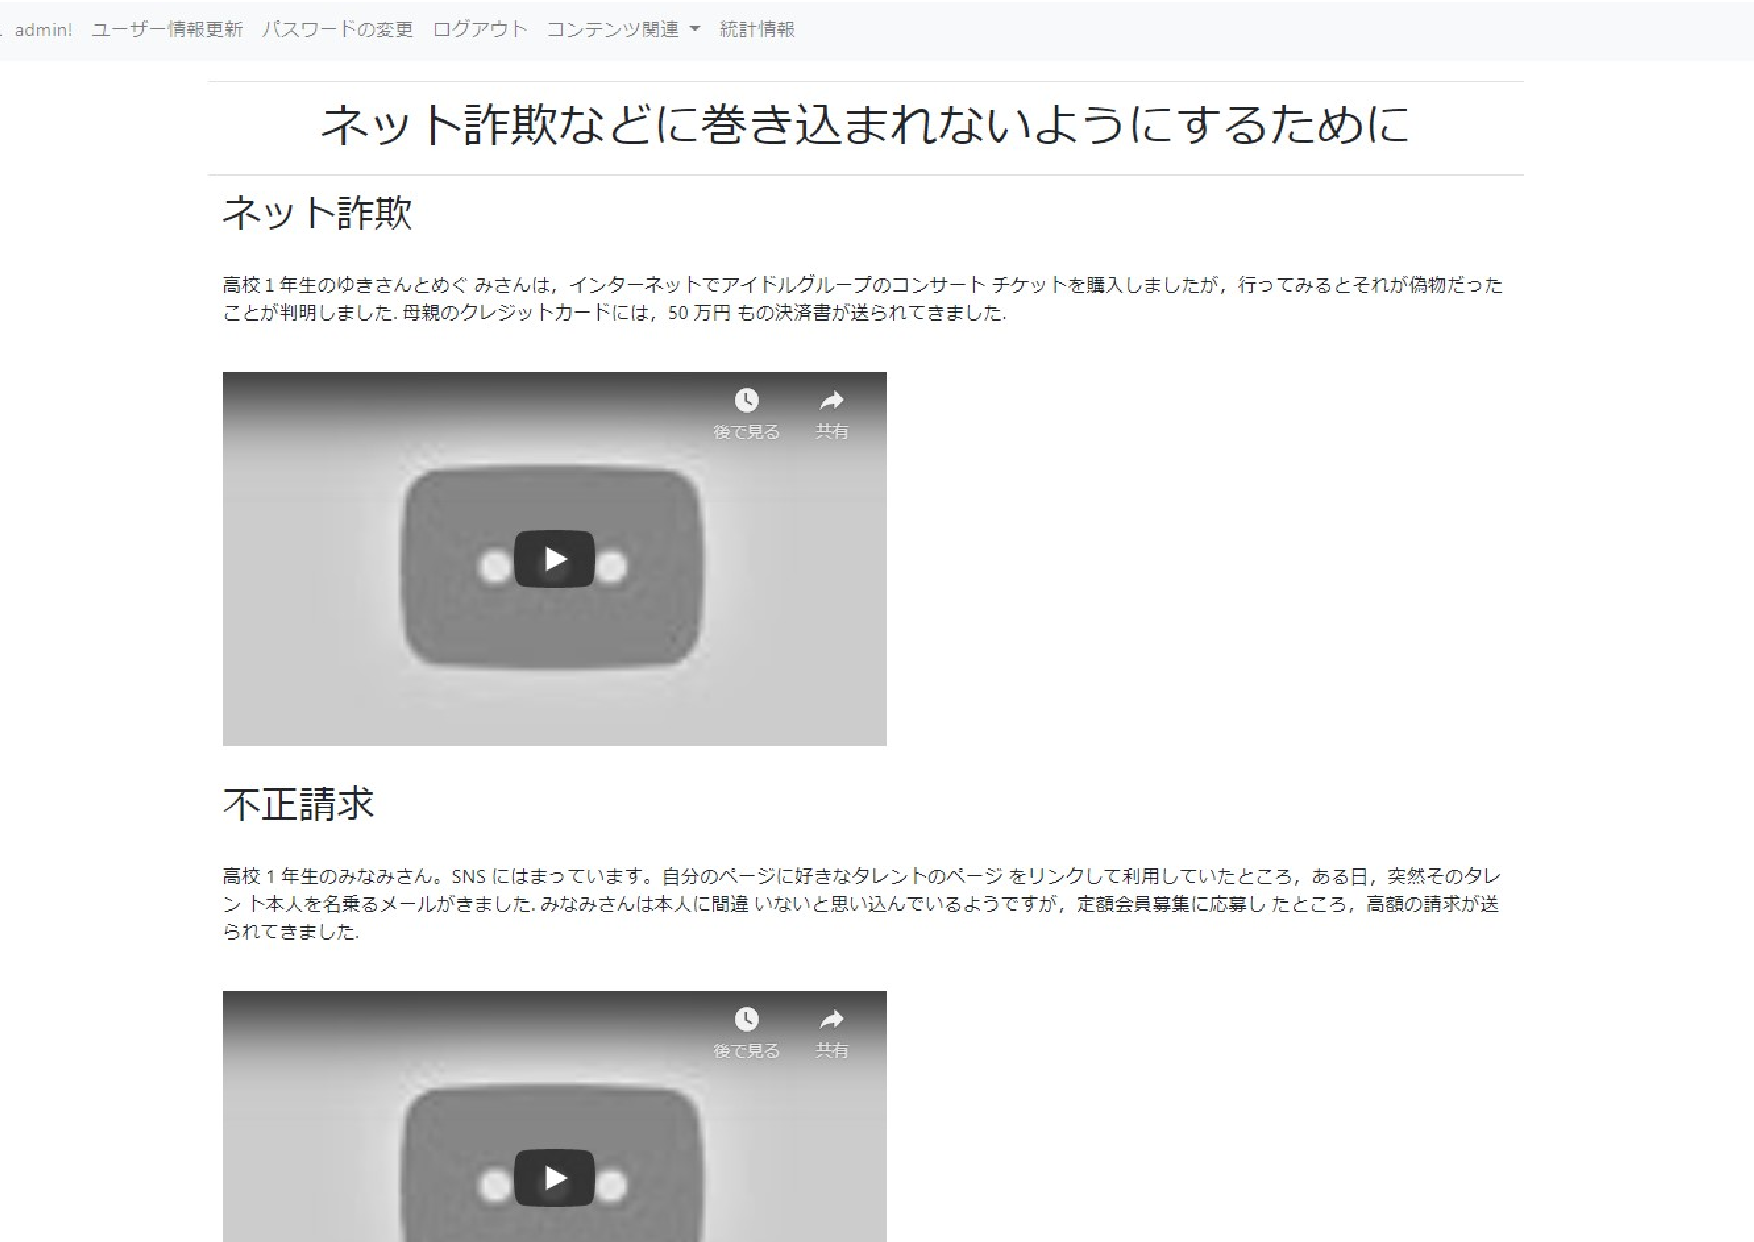
\includegraphics[width=18cm,height=17cm,keepaspectratio]{naiyou-crop.pdf}\\
        %includegraphicsの詳しい使い方ははLaTeXの参考書を参照.
    \end{center}
    \caption{コンテンツ閲覧時のGUI}
    \label{naiyou}
\end{figure}

\newpage
\subsubsection{システムの内部構成}
クライアントの内部構成を図\ref{client_naibu}に示す.はじめに,教材提供者および学習者が各々ネットワークに接続できる環境を用意し,Webブラウザを立ち上げ,特定のIPアドレスを入力しログインする.
ただし,教材提供者が本プラットフォームの機能を利用するにはログインは必須であるが,学習者は必須ではない.

Webブラウザで本プラットフォームに接続しログインした後,教材提供者はGUIのコンテンツ提供機能,統計情報提供機能,コンテナ管理機能を使用できる.
コンテンツ提供機能は教材提供者が入力した内容をサーバを介しデータベースに保存する.
統計情報提供機能はデータベースからサーバを介しデータを取得しWebブラウザ上に情報を表示する.
コンテナ管理機能は教材提供者が入力した内容をGoで作成したAPIで実行し,Dockerのコマンドを用いてコンテナが建ち上がっていることを確認し,建ち上がっていた場合それにアクセスするURLを画面上に発行する.

\begin{figure}[htbp]
    \begin{center}
        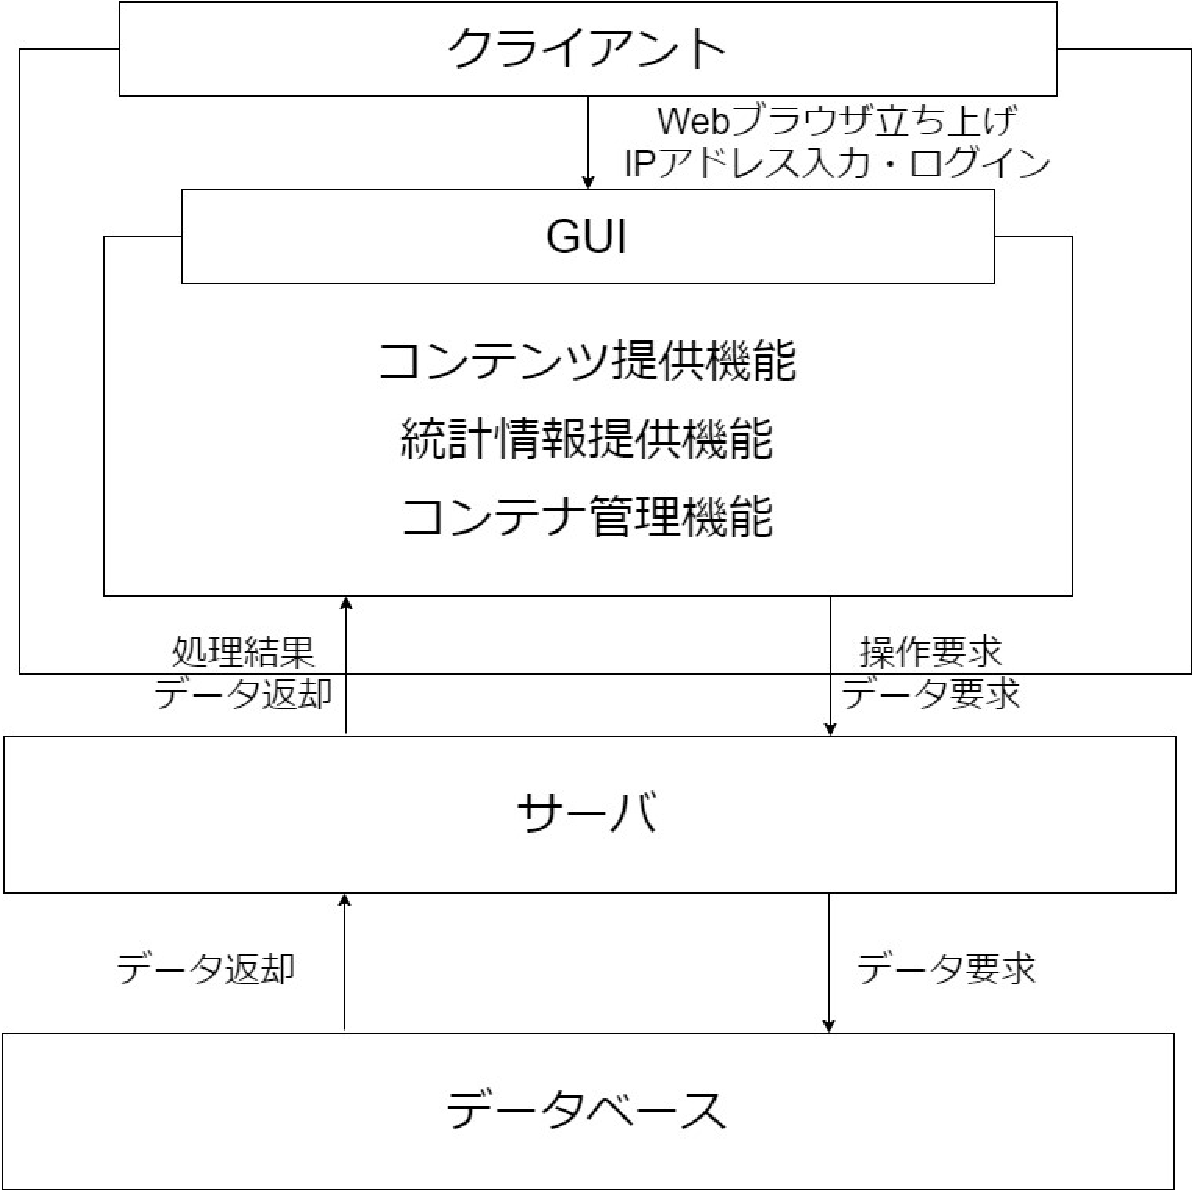
\includegraphics[width=13cm,height=12cm,keepaspectratio]{client_arch-crop.pdf}\\
        %includegraphicsの詳しい使い方ははLaTeXの参考書を参照.
    \end{center}
    \caption{クライアントの内部構成}
    \label{client_naibu}
\end{figure}

\newpage
続いて,サーバの内部構成を図\ref{server_naibu}に示す.サーバはDjangoを用いて作成されたDjango処理部とGoを用いて作成されたGo処理部,データを保存するためのデータベース処理部がある.
サーバはクライアントからの通信が行われた場合に動作する.それぞれの処理部の内容について以下に示す.

\begin{figure}[htbp]
    \begin{center}
        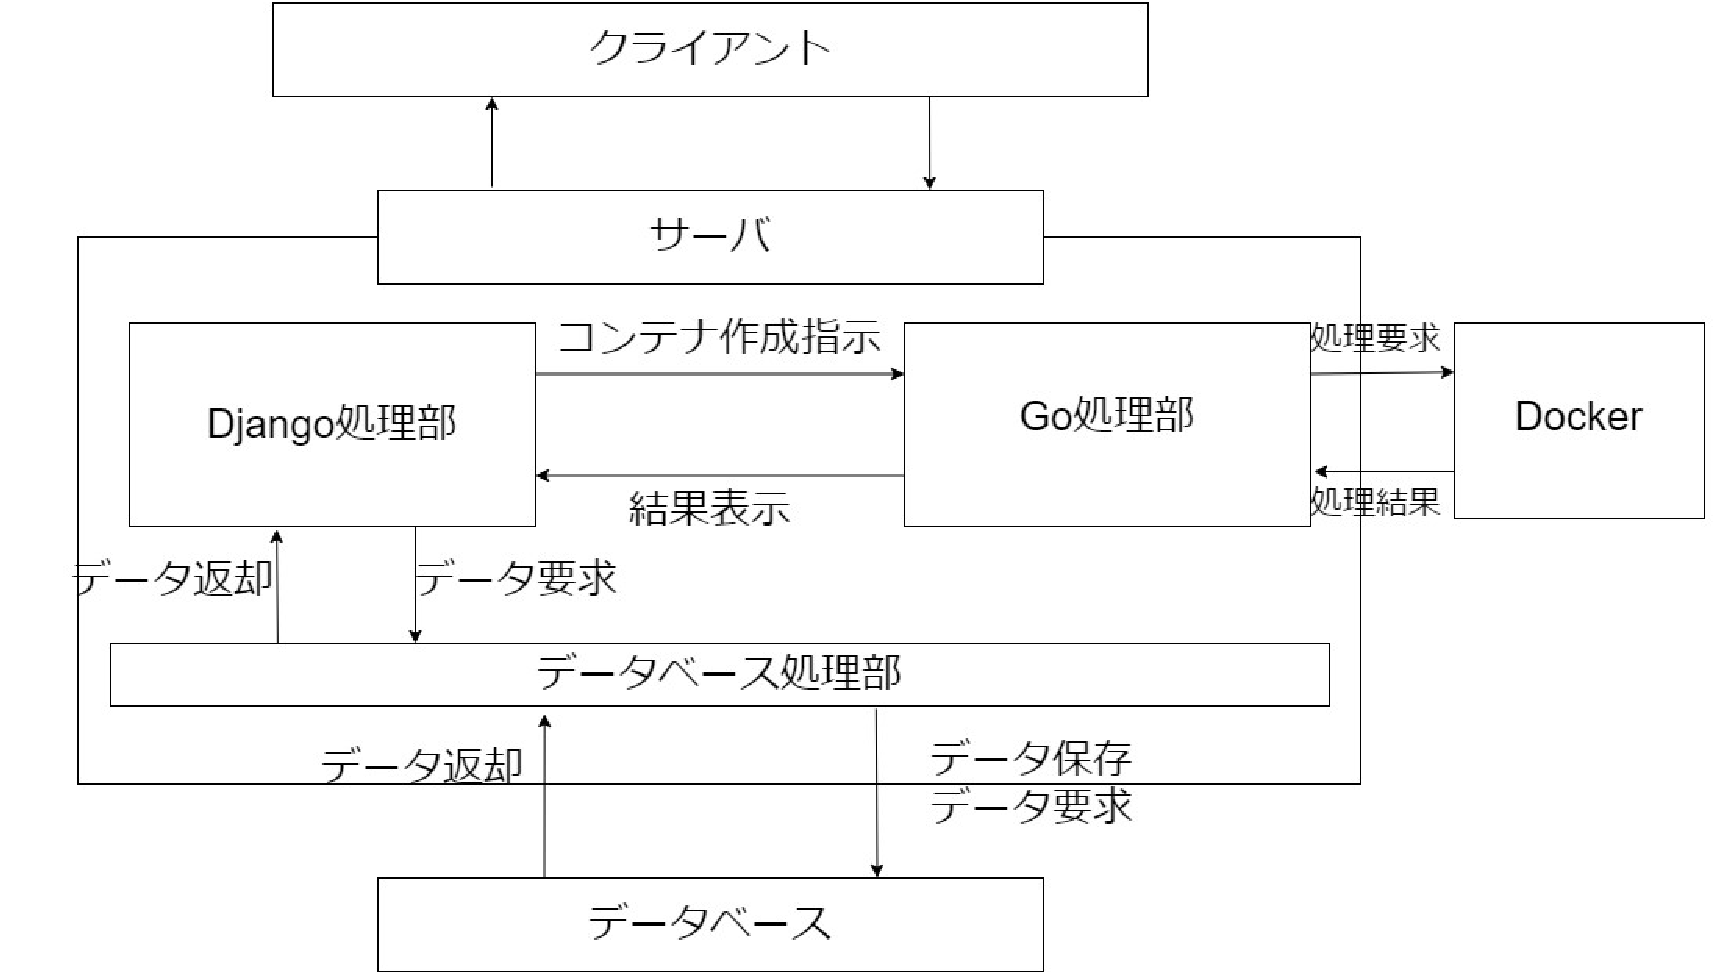
\includegraphics[width=17cm,height=16cm,keepaspectratio]{server_arch-crop.pdf}\\
        %includegraphicsの詳しい使い方ははLaTeXの参考書を参照.
    \end{center}
    \caption{サーバの内部構成}
    \label{server_naibu}
\end{figure}

\begin{description}
    \item[・Django処理部]\mbox{}\\
        Django処理部では,クライアントからフォームに従って入力されたデータをデータベースに登録,抽出する処理を行っている.
        具体的には,ユーザの新規登録,ログイン処理,パスワードや登録情報の変更,コンテンツ提供機能とコンテナ管理機能で入力された情報の登録と修正,タグの検索処理,統計情報提供機能のためのデータの検索が挙げられる.
    \item[・Go処理部]\mbox{}\\
        Go処理部では,コンテナ管理機能により入力された情報をAPIを用いてDockerに実行,処理させコンテナを建ち上げている.
    \item[・データベース処理部]\mbox{}\\
        データベース処理部では,Django処理部においてデータベースのやり取りが必要な場合に動作する.Django処理部からsqlコマンドが発行され,それを実行処理している.
\end{description}

\newpage
\subsubsection{システムのフローチャート}
教材提供者のフローチャートを図\ref{provider_flow}に,学習者のフローチャートを図\ref{learn_flow}に示す.本システムはまず,教材提供者はログインが必須,学習者は任意となっている.そのため今回は簡単のため教材提供者と学習者がともにログインした場合のフローチャートとする.

はじめに教材提供者について説明を行う.教材提供者は事前にユーザ登録を行ったことを管理者に通知し,管理者からアカウントを一般のものから教材提供者のアカウントに設定する必要がある.
教材提供者アカウントに設定した後,ログイン処理を行う.ログインが完了したら教材提供者はコンテンツ提供機能を用いてコンテンツの必要情報を入力し,サーバに対して登録を行う.
統計情報提供機能を用いる場合は,コンテンツに対する統計情報をサーバに対しリクエストすると,その結果が画面上に表示される.
コンテナ管理機能を用いる場合は,動作させたいアプリケーションの情報をクライアント上で入力することにより,サーバに対しその情報がリクエストされ,実行される.実行が正常に完了した場合,接続するためのURLが画面上に表示される.

\begin{figure}[htbp]
    \begin{center}
        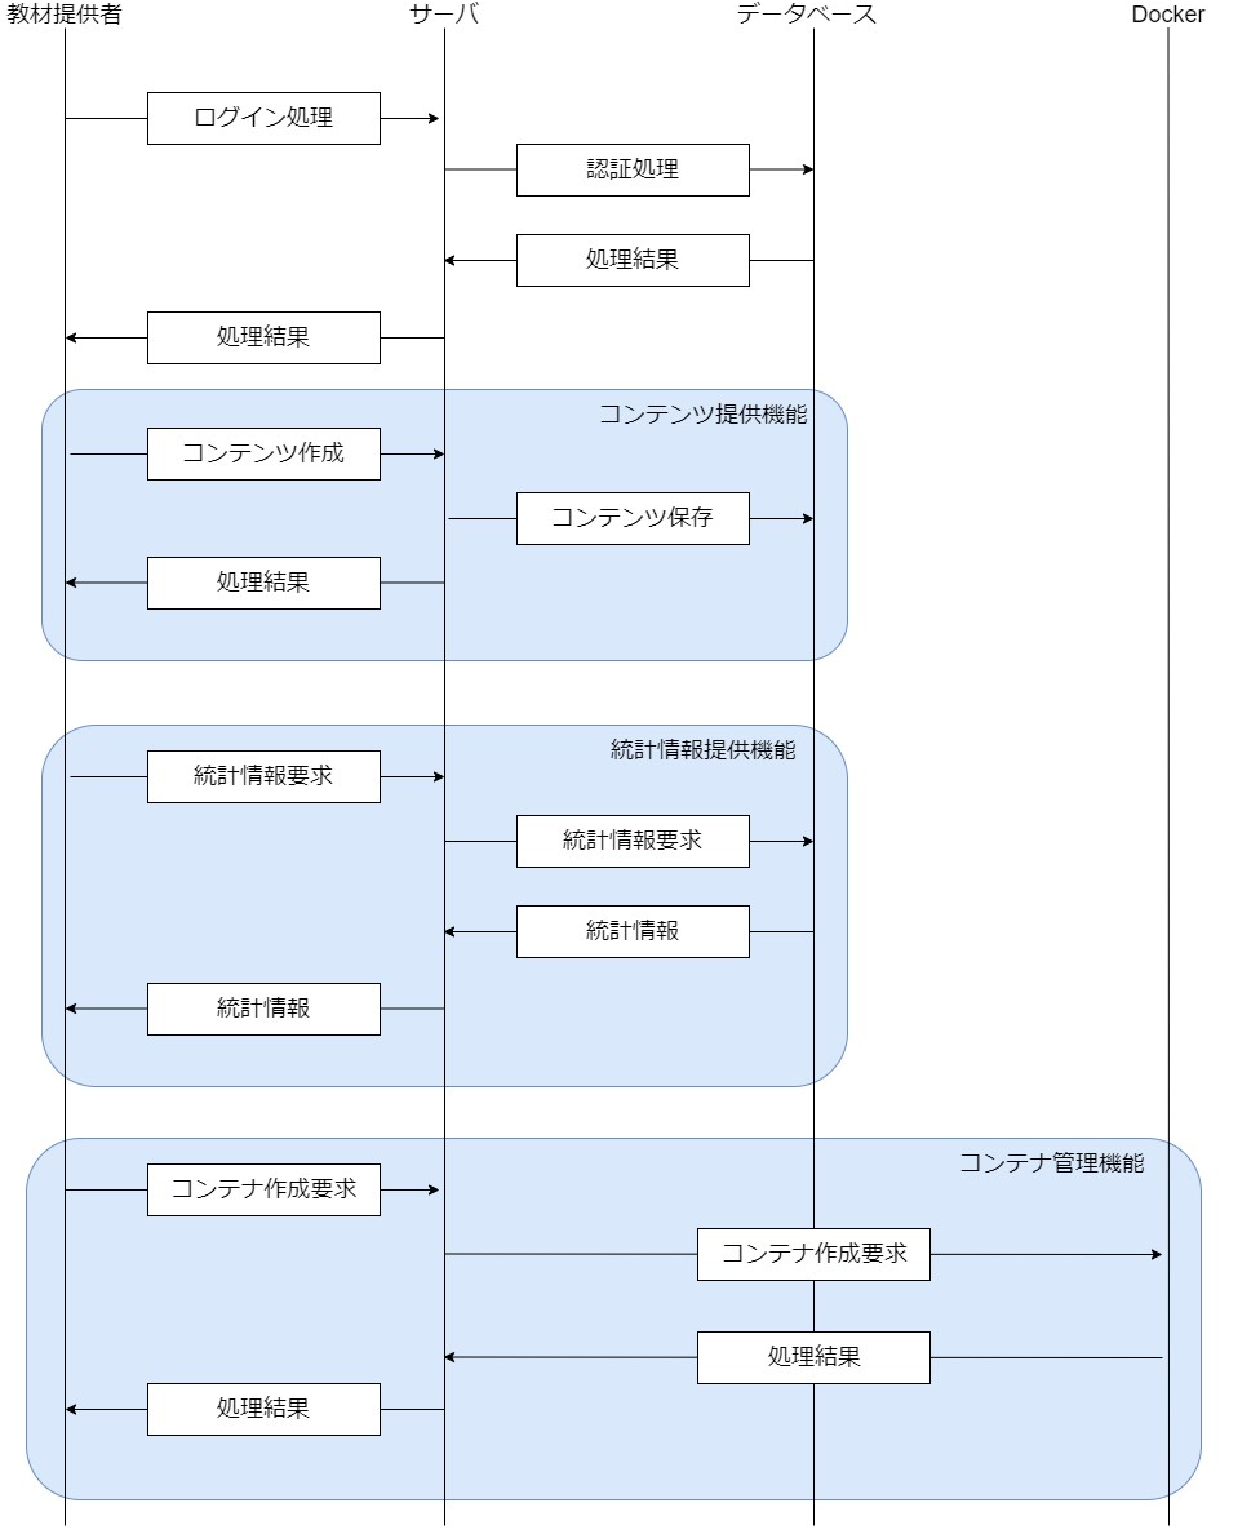
\includegraphics[width=15cm,height=14cm,keepaspectratio]{provider_flow-crop.pdf}\\
        %includegraphicsの詳しい使い方ははLaTeXの参考書を参照.
    \end{center}
    \caption{教材提供者のフローチャート}
    \label{provider_flow}
\end{figure}

\newpage
続いて学習者について説明を行う.学習者はWebブラウザで本プラットフォームに接続した後,本プラットフォームでアカウント作成を行うことができる.アカウント作成には,本プラットフォーム上で表示される
ユーザ名,性別,年齢,パスワードと確認用パスワードが必要である.アカウント作成後,トップページにて教材提供者が作成したコンテンツを選択,閲覧できる.

コンテンツ提供機能,統計情報提供機能,コンテナ管理機能についての詳細は\ref{sec:fun1}節,\ref{sec:fun2}節,\ref{sec:fun3}節にて述べる.

\begin{figure}[htbp]
    \begin{center}
        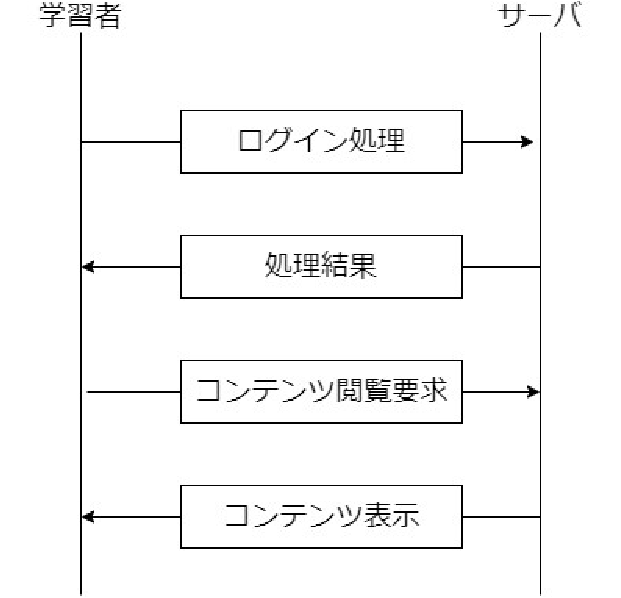
\includegraphics[width=13cm,height=12cm,keepaspectratio]{learn_flow-crop.pdf}\\
        %includegraphicsの詳しい使い方ははLaTeXの参考書を参照.
    \end{center}
    \caption{学習者のフローチャート}
    \label{learn_flow}
\end{figure}
\newpage
\subsection{コンテンツ提供機能}
日々変化する情報倫理に対応するために,コンテンツを素早く投稿,編集する必要がある.
それに対応するため,教材提供者が情報倫理に関するコンテンツをWebアプリケーション上で提供するためにコンテンツ提供機能を作成した.
本機能ではWeb上で教材提供者のみがコンテンツの投稿と管理ができる.
コンテンツを投稿する際のGUIを図\ref{content_teikyou}に示す.
図\ref{content_teikyou}に示したとおり,コンテンツを投稿する際に必要な情報は,コンテンツのタイトルとコンテンツのタグ,本文である.
本文はマークダウン形式で記入可能であり,画像や動画の挿入が容易にできる.またプレビュー機能もあるため投稿する前にどのような見た目で投稿されるのかを確認できる.

\begin{figure}[htbp]
    \begin{center}
        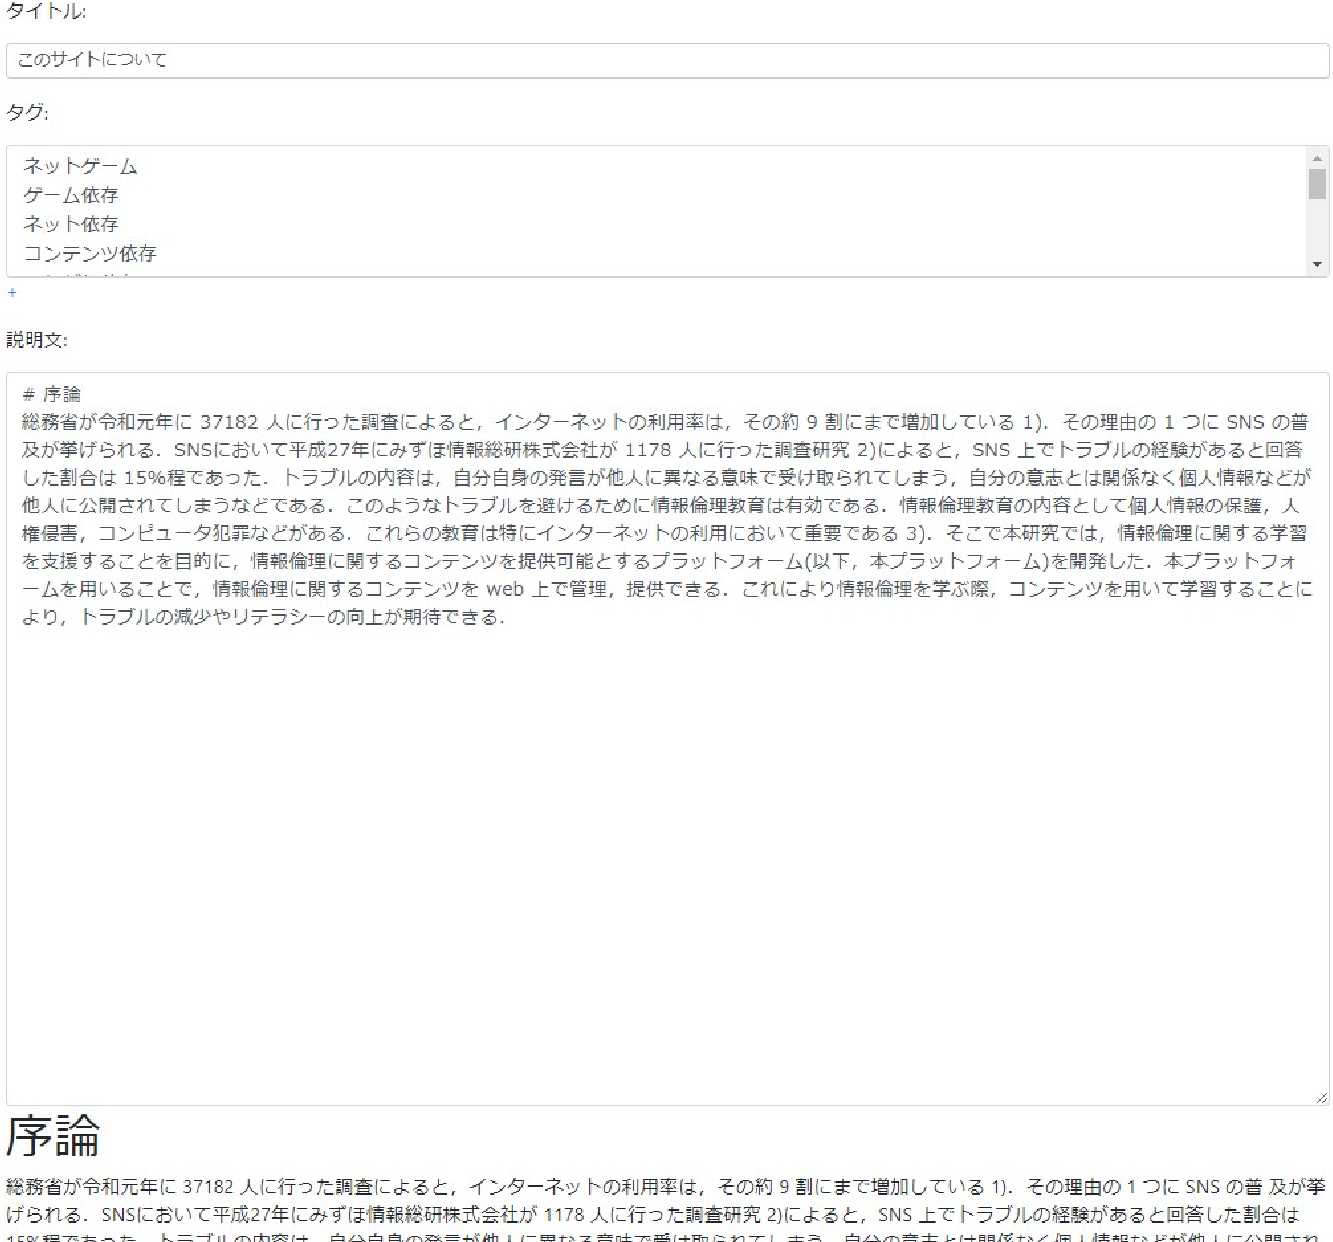
\includegraphics[width=16cm,height=15cm,keepaspectratio]{content_teikyou-crop.pdf}\\
        %includegraphicsの詳しい使い方ははLaTeXの参考書を参照.
    \end{center}
    \caption{コンテンツ提供機能のGUI}
    \label{content_teikyou}
\end{figure}

\newpage
コンテンツのタグは図\ref{content_teikyou}に示すプラスボタンを押下することにより,別画面で新たなタグを登録できる.
タグを登録する際のGUIを図\ref{tag}に示す.
\begin{figure}[htbp]
    \begin{center}
        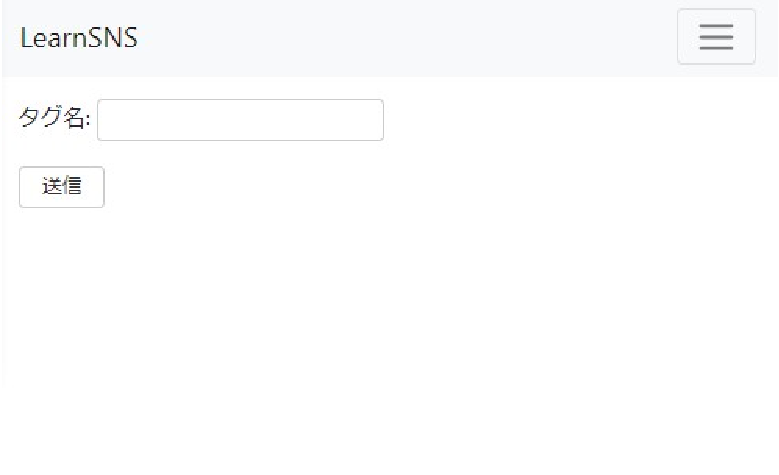
\includegraphics[width=13cm,height=12cm,keepaspectratio]{tag-crop.pdf}\\
        %includegraphicsの詳しい使い方ははLaTeXの参考書を参照.
    \end{center}
    \caption{タグ登録のGUI}
    \label{tag}
\end{figure}

\newpage
また,教材提供者はコンテンツを管理するためのグループに参加する.
そのグループはすべてのコンテンツに対して公開または非公開を選択することでコンテンツを管理する.
グループに参加している教材提供者全員が認可したコンテンツのみが学習者に公開される.
これにより,コンテンツの正当性を担保できる.
教材提供者をグループに参加させるには,図\ref{group_register}のようにして教材提供者のアカウントを選択し教材提供者のグループに登録する.

\begin{figure}[htbp]
    \begin{center}
        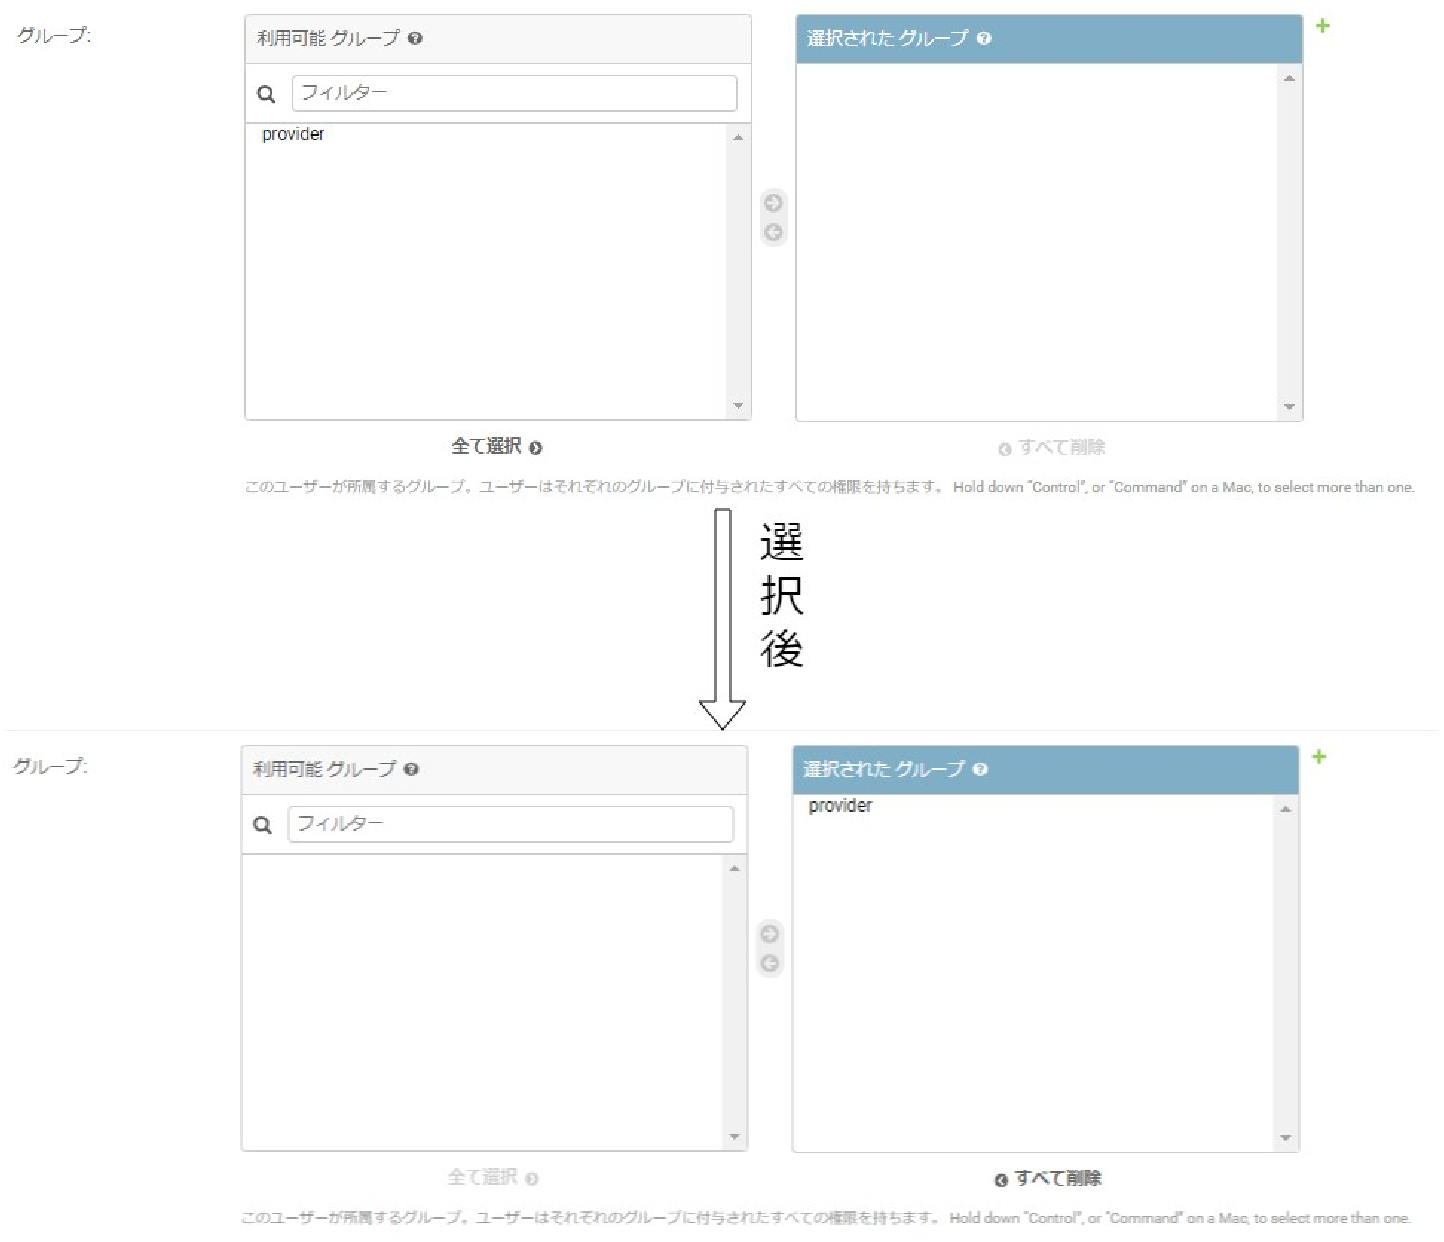
\includegraphics[width=16cm,height=15cm,keepaspectratio]{group_register-crop.pdf}\\
        %includegraphicsの詳しい使い方ははLaTeXの参考書を参照.
    \end{center}
    \caption{グループ登録のGUI}
    \label{group_register}
\end{figure}

\newpage
続いて本機能ではコンテンツ作成後にコンテンツの4択問題を作成することができる.問題の作成には,問題のタイトル,問題文,選択肢1~4および正解の選択肢をフォームに従って入力する.
問題作成の際のGUIを図\ref{create_question}に示す.

\begin{figure}[htbp]
    \begin{center}
        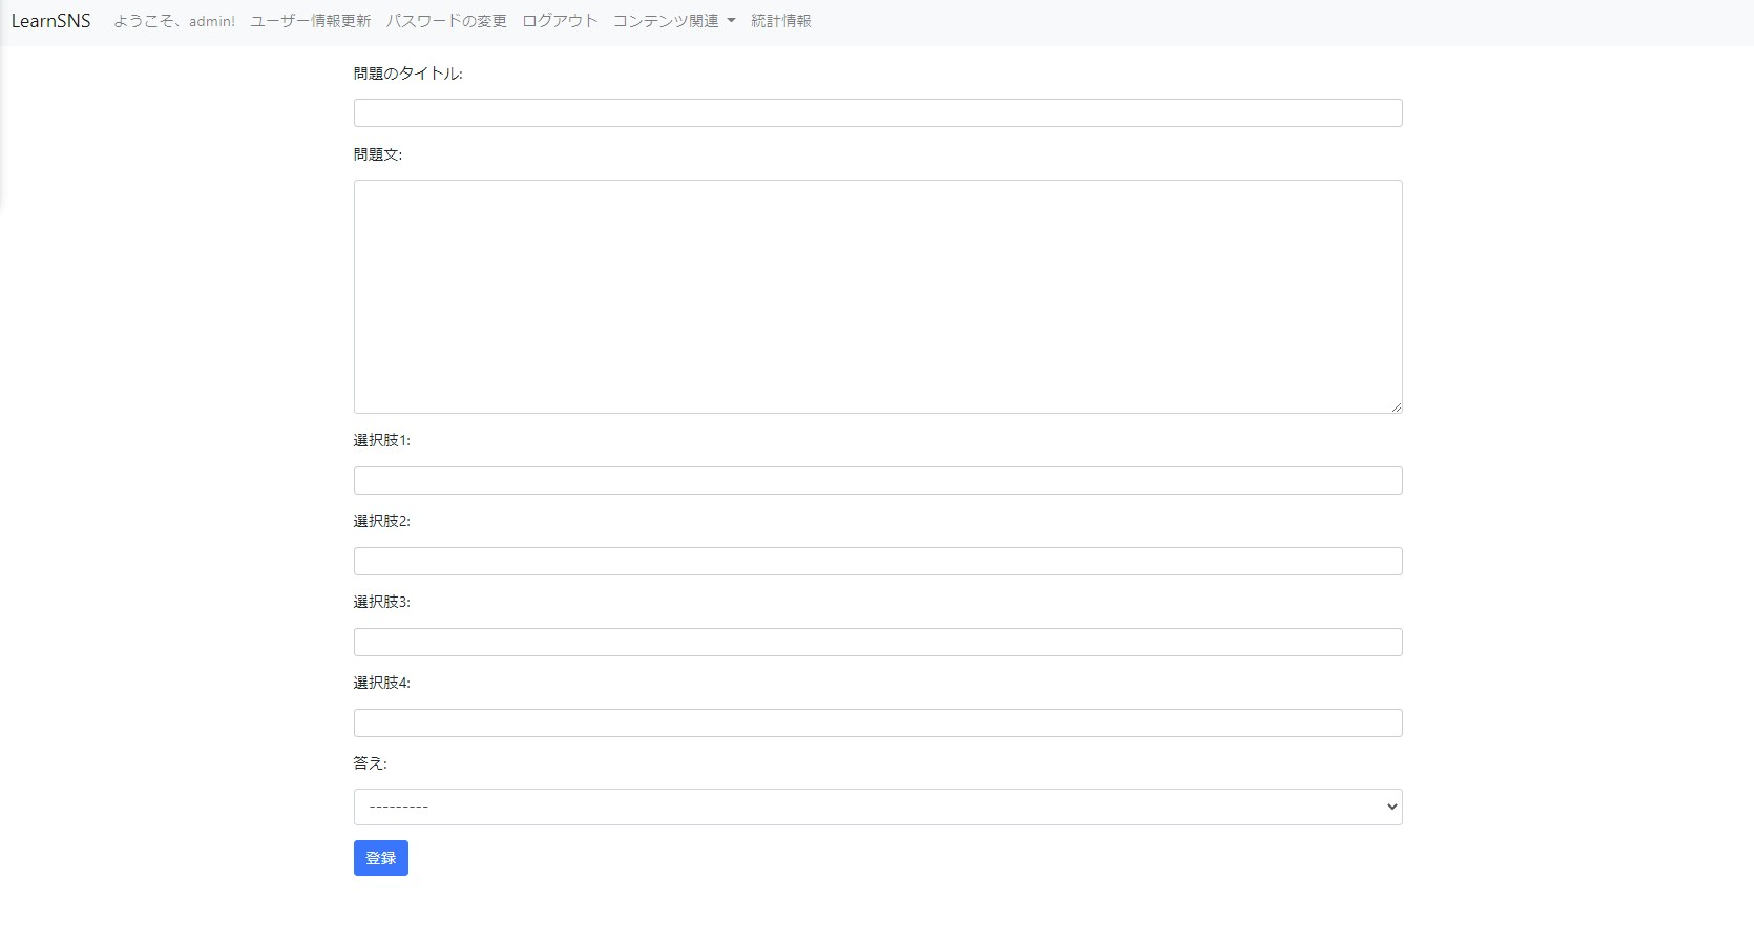
\includegraphics[width=18cm,height=17cm,keepaspectratio]{create_question-crop.pdf}\\
        %includegraphicsの詳しい使い方ははLaTeXの参考書を参照.
    \end{center}
    \caption{問題作成のGUI}
    \label{create_question}
\end{figure}

最後に,Djangoの機能を用いることにより本機能で投稿したコンテンツをJsonファイルに変換することができる.
Jsonファイルに変換するには,以下のような手順を経てコマンドを発行すればよい.
これにより,教材提供者はコンテンツを互いにJsonファイルを介して共有することが可能となる.

\begin{enumerate}
    \item 「docker exec -it コンテナ名 /bin/ash」などとして,本プラットフォームを動作させているコンテナにログインする.
    \item cdコマンドを用いてDjangoによって自動的に生成されたmanage.pyファイルと同階層に移動する.
    \item 「python manage.py dumpdata Jsonファイルに変換したいデータのDBのテーブル名 \textgreater 保存するJsonファイル名.json」を実行後,Jsonファイルが生成される.
\end{enumerate}
\subsection{統計情報提供機能}
統計情報提供機能は,教材提供者が作成した問題を学習者が解いた際の回答情報を基に,グラフで統計情報を提供する機能である.
これにより,教材提供者は作成したコンテンツの質を向上させることができる.
提示する統計情報の内容としては,問題の各選択肢における割合や回答者の年齢層,性別である.
統計情報提供機能のGUIは図\ref{toukei}の通りである.

\begin{figure}[htbp]
    \begin{center}
        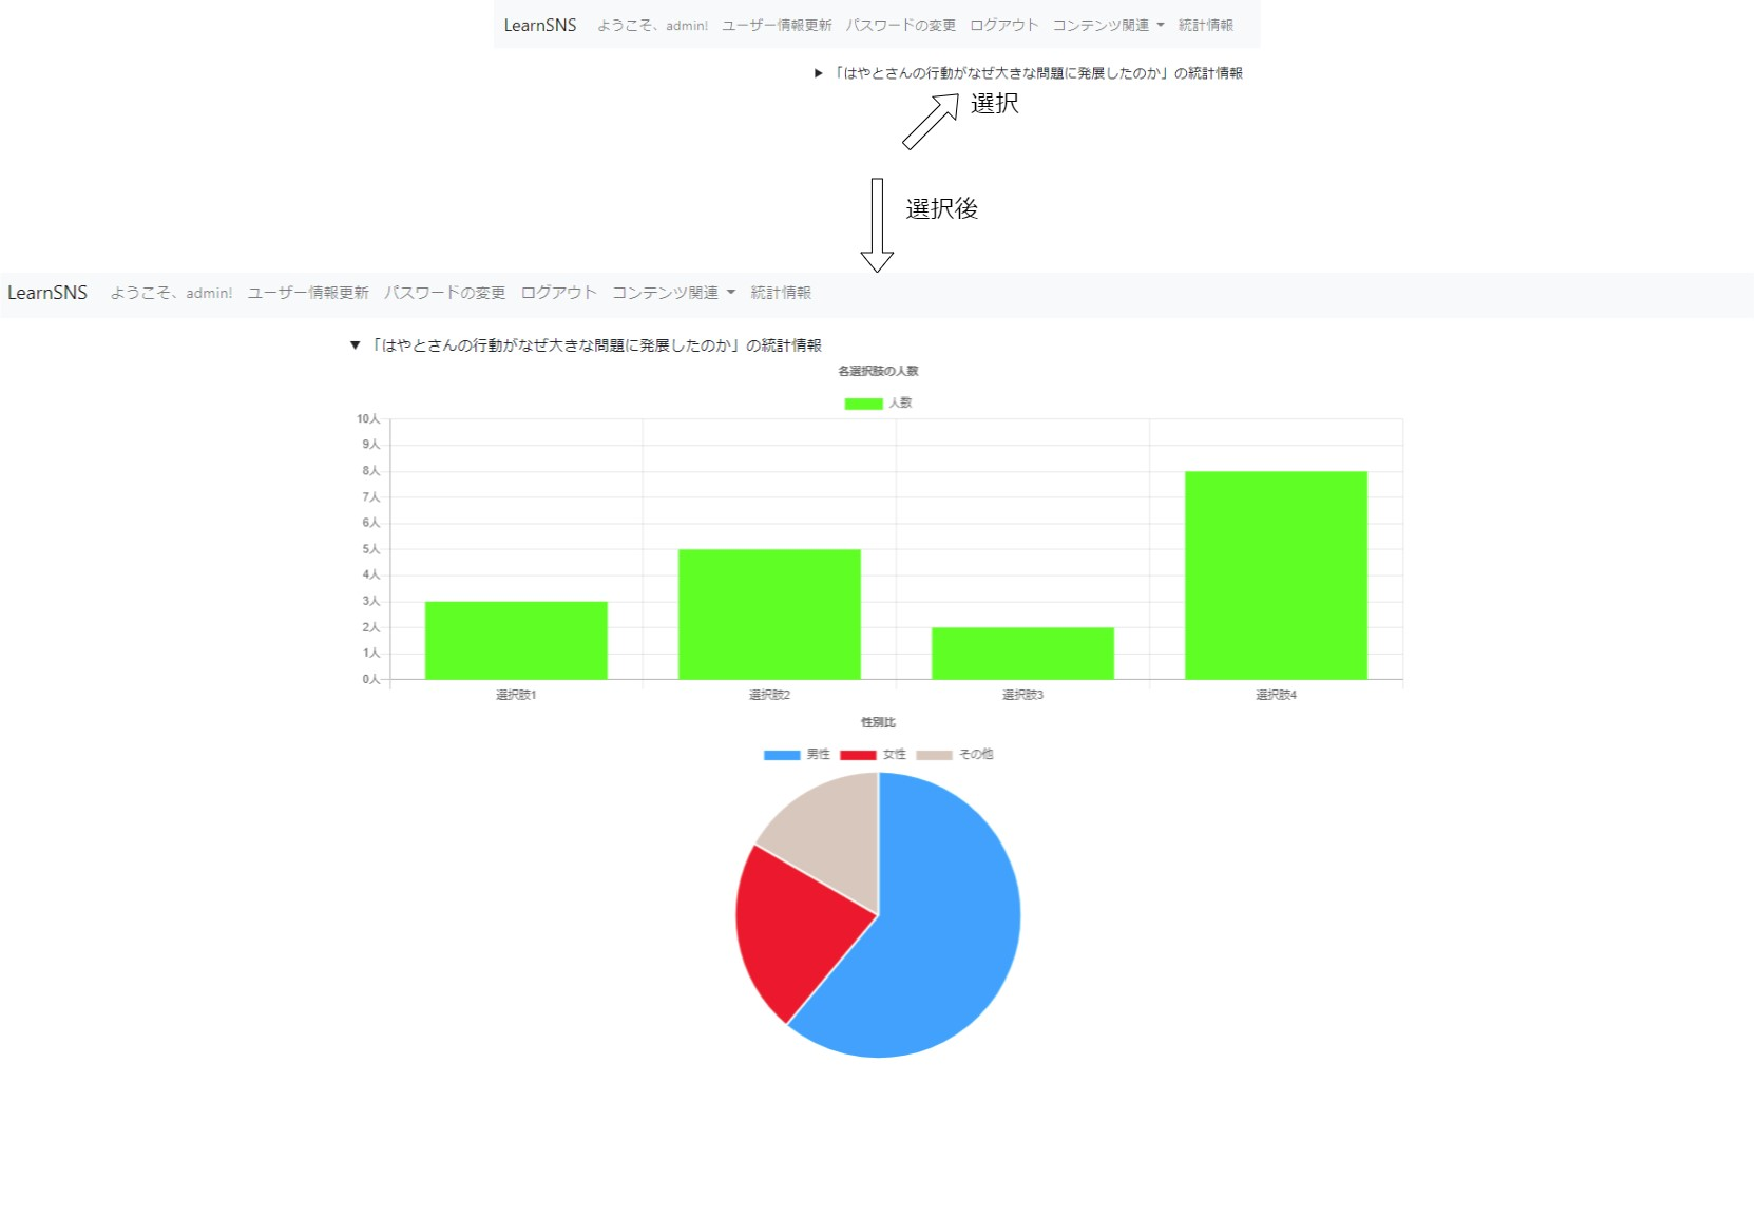
\includegraphics[width=15cm,height=14cm,keepaspectratio]{toukei_ex-crop.pdf}\\
        %includegraphicsの詳しい使い方ははLaTeXの参考書を参照.
    \end{center}
    \caption{統計情報提供機能のGUI}
    \label{toukei}
\end{figure}

\newpage
本機能はChart.jsというjavascriptで作成されたグラフ描画ライブラリを作成している.
Chart.jsでは線グラフ,棒グラフ,レーダーチャート,鶏頭図,ドーナツチャート,円グラフ,バブルチャートを作成できる.
本機能では,棒グラフと円グラフを使用している.

また,本機能で取得可能な情報を表\ref{info}に示す.
これらの取得できる情報を使って教材提供者はChart.jsで新たなグラフを挿入することができる.

\begin{table}[htb]
    \begin{center}
        \caption{取得可能情報一覧}
            \begin{tabular}{|l|l|} \hline
                取得可能情報 & 詳細 \\ \hline
                学習者情報 &   
                \begin{tabular}{l}
                    年齢\\性別\\回答した問題・選択肢 
                \end{tabular}\\ \hline
                コンテンツ情報 & 問題に対応したコンテンツ \\ \hline
            \end{tabular}
    \label{info}
    \end{center}
\end{table}
\subsection{コンテナ管理機能}
コンテナ管理機能は,教材提供者がDockerを用いて作成したアプリケーションを本プラットフォームでも利用可能とするための機能である.
本機能を利用するには,本プラットフォームで動作させたいコンテナ情報が記載されたDockerfile と docker-compose.yml を 事 前 にGithubなどのリポジトリに用意する.
そのURLと実行手順を本機能が提示するフォームに入力することにより,本プラットフォームで Docker のコンテナを作成し,アクセスするための URL を画面上に表示する.
教材提供者は発行された URL にアクセスすることで動作を確認できる.また,発行された URL をコンテンツ提供機能の本文に貼り付けることにより,学習者はそのコンテンツを利用できる.
ただし,作成したいコンテナが外部との通信のためにポートが必要な場合,使用ポートは本プラットフォームが提示するポートのみが使用可能である.